% Created 2023-02-07 Tue 13:17
% Intended LaTeX compiler: pdflatex
\documentclass[11pt]{article}
\usepackage[utf8]{inputenc}
\usepackage[T1]{fontenc}
\usepackage{graphicx}
\usepackage{longtable}
\usepackage{wrapfig}
\usepackage{rotating}
\usepackage[normalem]{ulem}
\usepackage{amsmath}
\usepackage{amssymb}
\usepackage{capt-of}
\usepackage{hyperref}
\date{\today}
\title{Matma}
\hypersetup{
 pdfauthor={},
 pdftitle={Matma},
 pdfkeywords={},
 pdfsubject={},
 pdfcreator={Emacs 30.0.50 (Org mode 9.6)}, 
 pdflang={English}}
\begin{document}

\maketitle
\tableofcontents


\section{liczby zespolone}
\label{sec:org2c876c8}
\begin{itemize}
\item \(\mathbb{Z}\) -- zbiór liczb całkowitych
\item \(\mathbb{R}\) -- zboór liczb rzeczywistych
\item \(\mathbb{C}\) -- zbiór liczb zespolonych
\end{itemize}
$$\mathbb{Z} \subset \mathbb{R} \subset \mathbb{C}$$
\subsection{postać algerbraiczna liczby zespolonej}
\label{sec:orgf42123a}
$$z=a+bi$$

\begin{itemize}
\item \(\Re(z) = a\) -- część rzeczywista liczby zespolonej.
\item \(\Im(z) = b\) -- częśc urojona liczby zespolonej.
\item \(i\) - jednostka urojona \(i^2=-1\)
\end{itemize}
\subsubsection{sprzężenie liczby zespolonej}
\label{sec:org475d921}
\begin{latex}
\begin{align*}
  z=a+bi && \overline{z}=a-bi \\
  w=f-gi && \overline{w}=f+gi \\
\end{align*}
\end{latex}

\subsection{postać trygonometryczna liczby zespolonej}
\label{sec:org95881db}
$$z=|z|(\cos\varphi \cdot \sin\varphi)$$
\subsection{postać wykładnicza liczby zespolonej}
\label{sec:orga791e5c}
$$z=|z| \cdot e^{i\varphi}$$
\subsection{moduł liczby zespolonej}
\label{sec:org80b4807}

\begin{center}
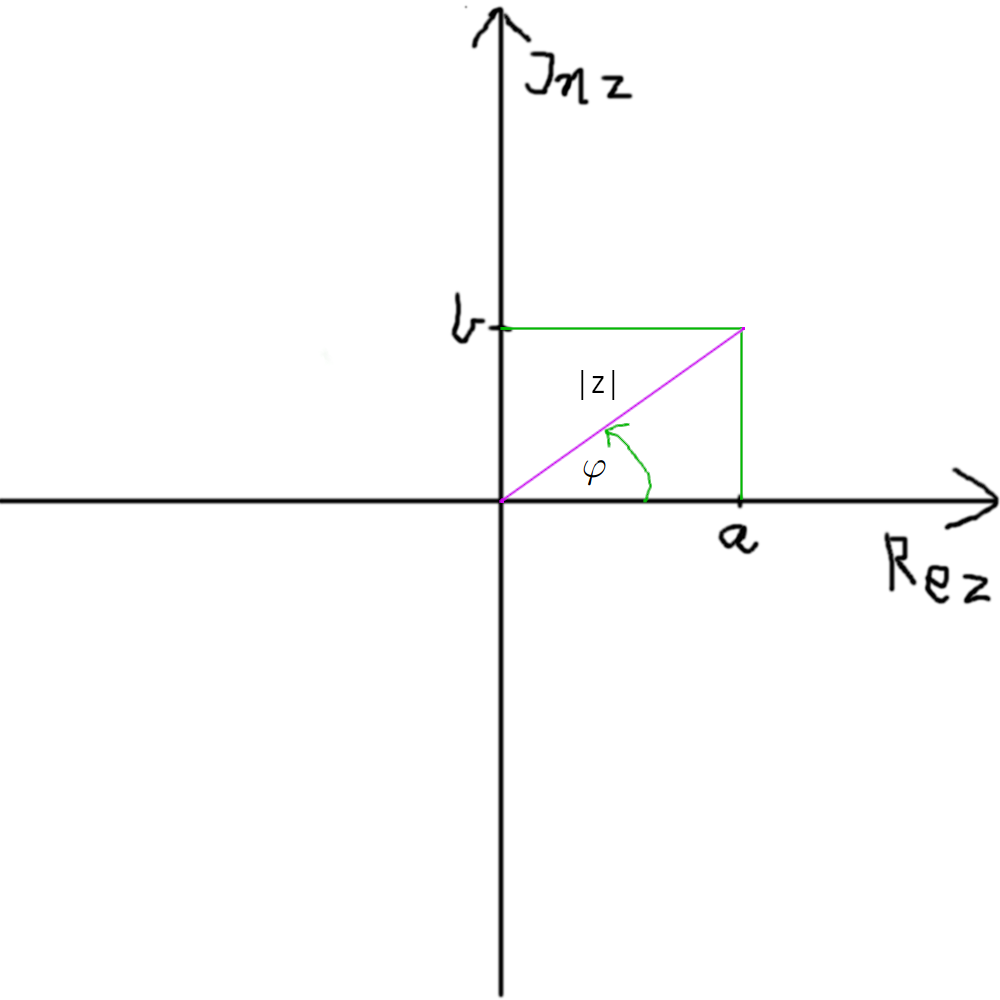
\includegraphics[width=.9\linewidth]{lzespolona.png}
\end{center}

$$|z|=\sqrt{a^2+b^2}$$

\(\varphi\) -- argument

\subsection{Potęgowanie liczby zespolonej}
\label{sec:org48cc8cb}
$$z=a+bi \to z=|z|(\cos \varphi + i \sin \varphi)^n \to |z|^n(\cos n \varphi + i \sin n \varphi)$$

\subsection{funkcja kwadratowa}
\label{sec:org34bbacb}
$$z^2+z+1=0$$
\(\Delta = b^2-4ac = -3\) -- brak rozwiązań w \(\mathbb{R}\)
$$\sqrt{\Delta} = \sqrt{-3} = \sqrt{(-1)3} = \sqrt{-1}  \sqrt{3} = \sqrt{i^2}\sqrt{3} = i \sqrt{3} $$
$$z_1 = \frac{-b - \sqrt{\Delta} }{2a} \lor z_2=\frac{-b + \sqrt{\Delta} }{2a}$$
$$z_1 = \frac{-1-i\sqrt{3}}{2} = -\frac{1}{2} + \frac{\sqrt{3}}{2}i \lor
z_2 = \frac{-1 + i\sqrt{3}}{2} = - \frac{1}{2}+ \frac{\sqrt{3}}{2}i $$
\section{Wektory}
\label{sec:orga49fbd4}
\subsection{Macierz obrotu}
\label{sec:org4694d33}
$$A = \begin{bmatrix}
        \cos \alpha & - \sin \alpha\\
        \sin \alpha & \cos \alpha\\
      \end{bmatrix}$$

\section{Stożkowe}
\label{sec:org9fa31da}
\[Q(\vec{x}) = a_{11}x_1^2 + 2a_{12}x_1x_2+a_{22}x_2^2
\to M =
\begin{bmatrix}
    a_{11} & a_{12}\\
    a_{21} & a_{22}\\
\end{bmatrix}\]

\(\det{M}\) -- wyróżnik formy kwadratowej \(Q(\vec{x})\)

\begin{latex}
\begin{align*}
  \det{M} &> 0 && \text{forma kwadratowa typu eliptycznego}\\
  \det{M} &= 0 && \text{forma kwadratowa typu parabolicznego}\\
  \det{M} &< 0 && \text{forma kwadratowa typu hiperbolicznego}\\
\end{align*}
\end{latex}

\subsection{Sprowadzanie do postaci kwadratowej}
\label{sec:org7db82a9}

\[Q(\vec{x}) = a_{11}x_1^2 + 2a_{12}x_1x_2+a_{22}x_2^}
\to
 Q(\vec{x}) = a_{1} \hat{x}_{1}^{2} + a_{2}\hat{x}_2^{2}\]

gdzie \(a_{1}, a_{2}\) -- wartości własne macierzy \(M\)

\(\hat{x}_1,\hat{x}_{2}\) -- współżędne wektora \(\vec{x}\) w nowej baze ortonormalnej \(\vec{v_{1}}, \vec{v_{2}}\) złożonej z wersorów własnych macierzy \(M\).

wersor własny -- wektor własny o długości 1.
\subsection{Elipsa}
\label{sec:org653c773}
\begin{description}
\item[{Wzór ogólny}] 
\end{description}
$$\frac{x_1^2}{a^2}+\frac{x_2^2}{b^2}=1$$
\begin{description}
\item[{Promienie}] 
\end{description}
\(a,b\)
\subsection{Parabola}
\label{sec:orgdf5bb55}
\begin{description}
\item[{Wzór ogólny}] $$x_1=ax_2^2$$
\end{description}
\subsection{Hiperbola}
\label{sec:org3fbeb6d}
\begin{description}
\item[{Wzór ogólny}] 
\end{description}
$$\frac{x_1^2}{a^2}-\frac{x_2^2}{b^2}=1$$
\begin{description}
\item[{Wieszchołki}] $$x_1 = \pm a$$
\item[{Asymptoty}] $$x_2 = \pm \frac{b}{a}x_1$$
\end{description}

\section{\(\mathbb{R}^3\)}
\label{sec:org40abd4e}
\subsection{Równianie ogólne płaszczyzny}
\label{sec:orgc4eae3a}

\begin{center}
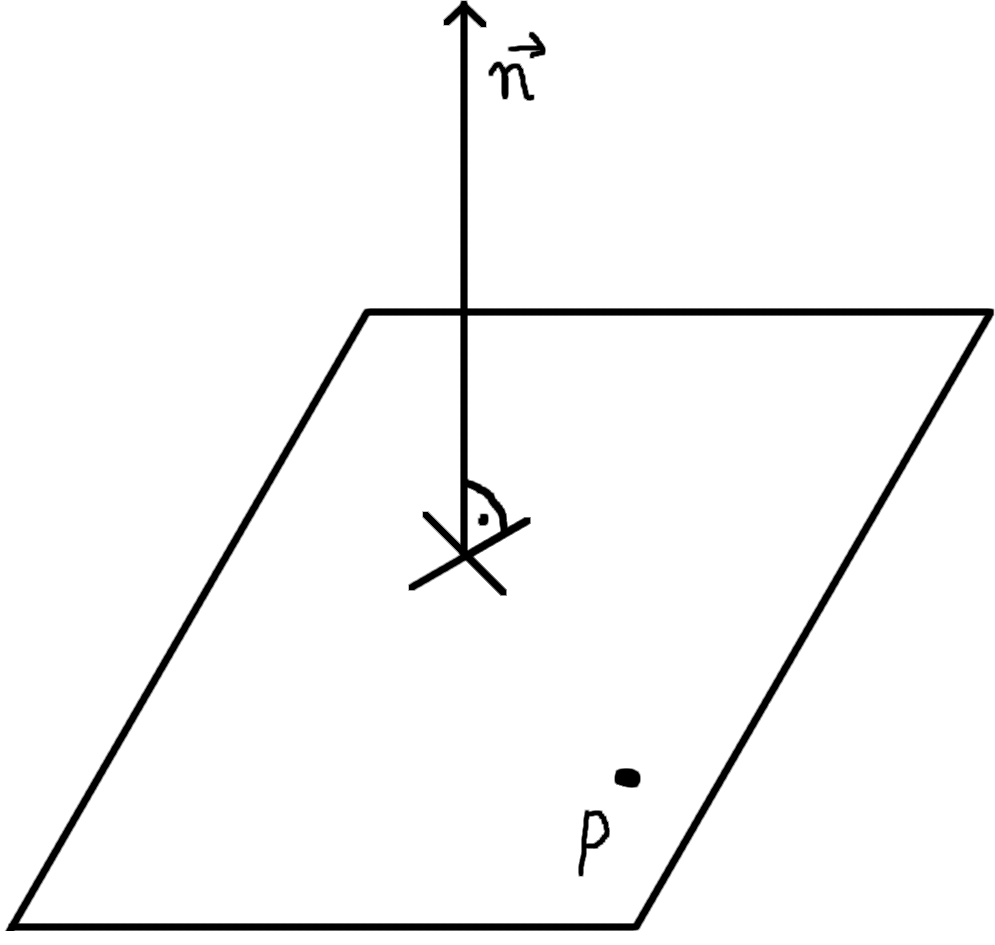
\includegraphics[width=.9\linewidth]{figures/plaszczyzna.png}
\end{center}

\begin{latex}
\begin{align*}
\vec{n}=[A,B,C] && P=(x_{0}, y_{0}, z_{0})
\end{align*}
\end{latex}

$$A(x - x_{0}) + B(y-y_{0}) + C(z - z_{0}) = 0$$
\section{Analiza}
\label{sec:org6b20976}
\subsection{Wzór Taylora}
\label{sec:org1dfecef}
\[f(x) \approx f(x_{0}) +
  \frac{f'(x_0)}{1!}(x - x_0)^1 +
  \frac{f''(x_0)}{2!}(x - x_0)^2 +
  \ldots +
  \frac{f^{(n-1)}'(x_0)}{(n-1)!}(x - x_0)^{(n-1)} +
  \underbrace{\frac{f^{(n)}'(x_0)}{n!}(x - x_0)^n}_{\text{reszta}}
   \]
\subsection{Asymptoty}
\label{sec:orgd97632e}
\subsubsection{Pionowe}
\label{sec:org5c03cd5}
\begin{itemize}
\item Prawostronna w punkcie \(p\)
jeżeli \(\lim_{x \to p^+} = - \infty\).
\item Lewostronna w punkcie \(p\)
jeżeli \(\lim_{x \to p^-} = + \infty\).
\item Obustronna  jeżeli oba powyższe.
\end{itemize}
\subsubsection{Ukośne}
\label{sec:org4c5e5fd}
\begin{latex}
\begin{align*}
  & y = ax +b
  && a = \lim_{x \to \pm \infty} \frac{f(x)}{x}
  && b = \lim_{x \to \pm \infty } \left( f(x) -ax \right)
\end{align*}
\end{latex}
Jeżeli \(a = 0\) jest to asymptota pozioma.
\end{document}